% Created by tikzDevice version 0.10.1 on 2017-03-17 16:56:45
% !TEX encoding = UTF-8 Unicode
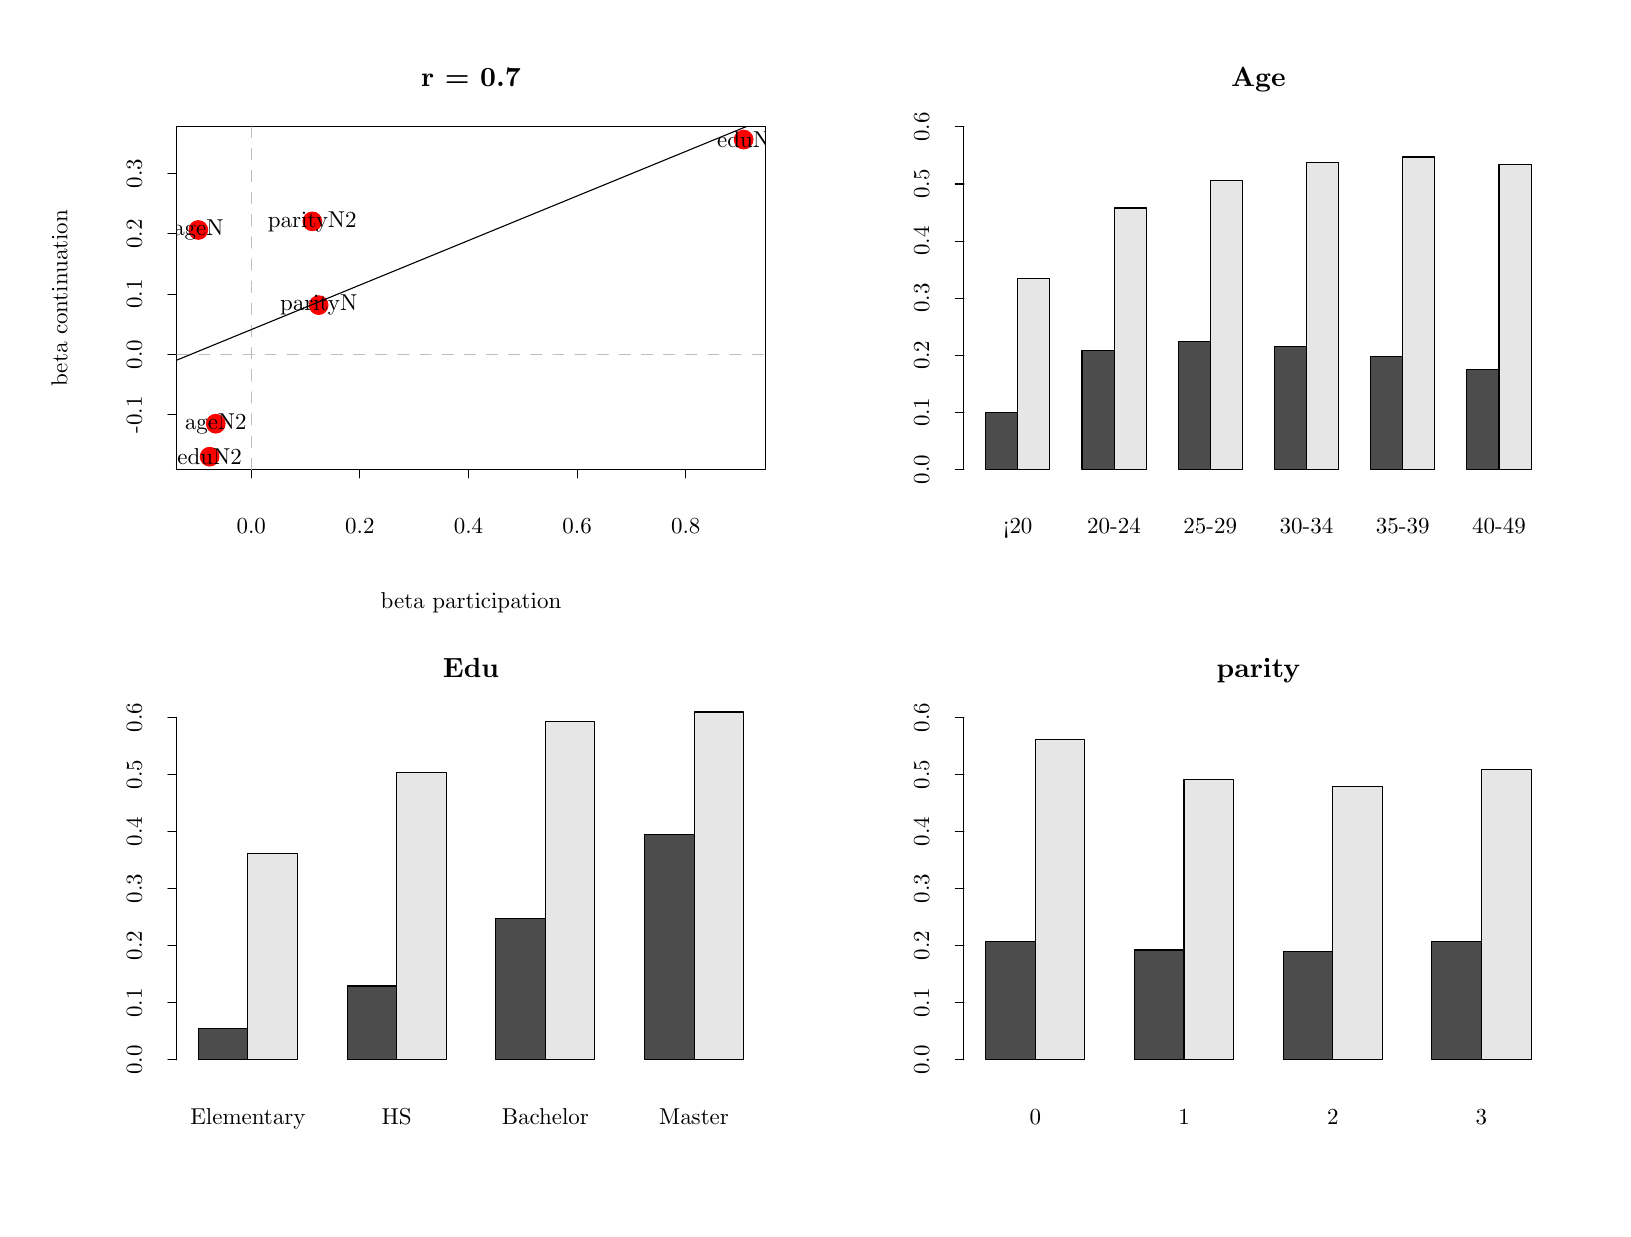
\begin{tikzpicture}[x=1pt,y=1pt]
\definecolor{fillColor}{RGB}{255,255,255}
\path[use as bounding box,fill=fillColor,fill opacity=0.00] (0,0) rectangle (569.06,426.79);
\begin{scope}
\path[clip] ( 53.78,267.18) rectangle (266.60,390.94);
\definecolor{drawColor}{RGB}{255,0,0}
\definecolor{fillColor}{RGB}{255,0,0}

\path[draw=drawColor,line width= 0.4pt,line join=round,line cap=round,fill=fillColor] ( 61.67,353.68) circle (  3.36);

\path[draw=drawColor,line width= 0.4pt,line join=round,line cap=round,fill=fillColor] (105.15,326.53) circle (  3.36);

\path[draw=drawColor,line width= 0.4pt,line join=round,line cap=round,fill=fillColor] (258.72,386.35) circle (  3.36);

\path[draw=drawColor,line width= 0.4pt,line join=round,line cap=round,fill=fillColor] ( 65.75,271.76) circle (  3.36);

\path[draw=drawColor,line width= 0.4pt,line join=round,line cap=round,fill=fillColor] ( 67.96,283.68) circle (  3.36);

\path[draw=drawColor,line width= 0.4pt,line join=round,line cap=round,fill=fillColor] (102.86,356.80) circle (  3.36);
\end{scope}
\begin{scope}
\path[clip] (  0.00,  0.00) rectangle (569.06,426.79);
\definecolor{drawColor}{RGB}{0,0,0}

\path[draw=drawColor,line width= 0.4pt,line join=round,line cap=round] ( 80.80,267.18) -- (237.80,267.18);

\path[draw=drawColor,line width= 0.4pt,line join=round,line cap=round] ( 80.80,267.18) -- ( 80.80,264.09);

\path[draw=drawColor,line width= 0.4pt,line join=round,line cap=round] (120.05,267.18) -- (120.05,264.09);

\path[draw=drawColor,line width= 0.4pt,line join=round,line cap=round] (159.30,267.18) -- (159.30,264.09);

\path[draw=drawColor,line width= 0.4pt,line join=round,line cap=round] (198.55,267.18) -- (198.55,264.09);

\path[draw=drawColor,line width= 0.4pt,line join=round,line cap=round] (237.80,267.18) -- (237.80,264.09);

\node[text=drawColor,anchor=base,inner sep=0pt, outer sep=0pt, scale=  0.83] at ( 80.80,243.87) {0.0};

\node[text=drawColor,anchor=base,inner sep=0pt, outer sep=0pt, scale=  0.83] at (120.05,243.87) {0.2};

\node[text=drawColor,anchor=base,inner sep=0pt, outer sep=0pt, scale=  0.83] at (159.30,243.87) {0.4};

\node[text=drawColor,anchor=base,inner sep=0pt, outer sep=0pt, scale=  0.83] at (198.55,243.87) {0.6};

\node[text=drawColor,anchor=base,inner sep=0pt, outer sep=0pt, scale=  0.83] at (237.80,243.87) {0.8};

\path[draw=drawColor,line width= 0.4pt,line join=round,line cap=round] ( 53.78,286.89) -- ( 53.78,374.09);

\path[draw=drawColor,line width= 0.4pt,line join=round,line cap=round] ( 53.78,286.89) -- ( 50.69,286.89);

\path[draw=drawColor,line width= 0.4pt,line join=round,line cap=round] ( 53.78,308.69) -- ( 50.69,308.69);

\path[draw=drawColor,line width= 0.4pt,line join=round,line cap=round] ( 53.78,330.49) -- ( 50.69,330.49);

\path[draw=drawColor,line width= 0.4pt,line join=round,line cap=round] ( 53.78,352.29) -- ( 50.69,352.29);

\path[draw=drawColor,line width= 0.4pt,line join=round,line cap=round] ( 53.78,374.09) -- ( 50.69,374.09);

\node[text=drawColor,rotate= 90.00,anchor=base,inner sep=0pt, outer sep=0pt, scale=  0.83] at ( 41.23,286.89) {-0.1};

\node[text=drawColor,rotate= 90.00,anchor=base,inner sep=0pt, outer sep=0pt, scale=  0.83] at ( 41.23,308.69) {0.0};

\node[text=drawColor,rotate= 90.00,anchor=base,inner sep=0pt, outer sep=0pt, scale=  0.83] at ( 41.23,330.49) {0.1};

\node[text=drawColor,rotate= 90.00,anchor=base,inner sep=0pt, outer sep=0pt, scale=  0.83] at ( 41.23,352.29) {0.2};

\node[text=drawColor,rotate= 90.00,anchor=base,inner sep=0pt, outer sep=0pt, scale=  0.83] at ( 41.23,374.09) {0.3};

\path[draw=drawColor,line width= 0.4pt,line join=round,line cap=round] ( 53.78,267.18) --
	(266.60,267.18) --
	(266.60,390.94) --
	( 53.78,390.94) --
	( 53.78,267.18);
\end{scope}
\begin{scope}
\path[clip] (  0.00,213.40) rectangle (284.53,426.79);
\definecolor{drawColor}{RGB}{0,0,0}

\node[text=drawColor,anchor=base,inner sep=0pt, outer sep=0pt, scale=  1.00] at (160.19,405.43) {\bfseries r = 0.7};

\node[text=drawColor,anchor=base,inner sep=0pt, outer sep=0pt, scale=  0.83] at (160.19,216.98) {beta participation};

\node[text=drawColor,rotate= 90.00,anchor=base,inner sep=0pt, outer sep=0pt, scale=  0.83] at ( 14.34,329.06) {beta continuation};
\end{scope}
\begin{scope}
\path[clip] ( 53.78,267.18) rectangle (266.60,390.94);
\definecolor{drawColor}{RGB}{0,0,0}

\node[text=drawColor,anchor=base,inner sep=0pt, outer sep=0pt, scale=  0.83] at ( 61.67,351.63) {ageN};

\node[text=drawColor,anchor=base,inner sep=0pt, outer sep=0pt, scale=  0.83] at (105.15,324.48) {parityN};

\node[text=drawColor,anchor=base,inner sep=0pt, outer sep=0pt, scale=  0.83] at (258.72,383.49) {eduN};

\node[text=drawColor,anchor=base,inner sep=0pt, outer sep=0pt, scale=  0.83] at ( 65.75,268.91) {eduN2};

\node[text=drawColor,anchor=base,inner sep=0pt, outer sep=0pt, scale=  0.83] at ( 67.96,281.63) {ageN2};

\node[text=drawColor,anchor=base,inner sep=0pt, outer sep=0pt, scale=  0.83] at (102.86,354.75) {parityN2};
\definecolor{drawColor}{RGB}{190,190,190}

\path[draw=drawColor,line width= 0.4pt,dash pattern=on 4pt off 4pt ,line join=round,line cap=round] ( 53.78,308.69) -- (266.60,308.69);

\path[draw=drawColor,line width= 0.4pt,dash pattern=on 4pt off 4pt ,line join=round,line cap=round] ( 80.80,267.18) -- ( 80.80,390.94);
\definecolor{drawColor}{RGB}{0,0,0}

\path[draw=drawColor,line width= 0.4pt,line join=round,line cap=round] ( 53.78,306.61) -- (266.60,393.88);
\end{scope}
\begin{scope}
\path[clip] (284.53,213.40) rectangle (569.06,426.79);
\definecolor{drawColor}{RGB}{0,0,0}
\definecolor{fillColor}{gray}{0.30}

\path[draw=drawColor,line width= 0.4pt,line join=round,line cap=round,fill=fillColor] (346.19,267.18) rectangle (357.78,287.71);
\definecolor{fillColor}{RGB}{230,230,230}

\path[draw=drawColor,line width= 0.4pt,line join=round,line cap=round,fill=fillColor] (357.78,267.18) rectangle (369.38,336.10);
\definecolor{fillColor}{gray}{0.30}

\path[draw=drawColor,line width= 0.4pt,line join=round,line cap=round,fill=fillColor] (380.97,267.18) rectangle (392.56,309.98);
\definecolor{fillColor}{RGB}{230,230,230}

\path[draw=drawColor,line width= 0.4pt,line join=round,line cap=round,fill=fillColor] (392.56,267.18) rectangle (404.15,361.62);
\definecolor{fillColor}{gray}{0.30}

\path[draw=drawColor,line width= 0.4pt,line join=round,line cap=round,fill=fillColor] (415.74,267.18) rectangle (427.33,313.54);
\definecolor{fillColor}{RGB}{230,230,230}

\path[draw=drawColor,line width= 0.4pt,line join=round,line cap=round,fill=fillColor] (427.33,267.18) rectangle (438.92,371.72);
\definecolor{fillColor}{gray}{0.30}

\path[draw=drawColor,line width= 0.4pt,line join=round,line cap=round,fill=fillColor] (450.51,267.18) rectangle (462.11,311.59);
\definecolor{fillColor}{RGB}{230,230,230}

\path[draw=drawColor,line width= 0.4pt,line join=round,line cap=round,fill=fillColor] (462.11,267.18) rectangle (473.70,378.18);
\definecolor{fillColor}{gray}{0.30}

\path[draw=drawColor,line width= 0.4pt,line join=round,line cap=round,fill=fillColor] (485.29,267.18) rectangle (496.88,308.11);
\definecolor{fillColor}{RGB}{230,230,230}

\path[draw=drawColor,line width= 0.4pt,line join=round,line cap=round,fill=fillColor] (496.88,267.18) rectangle (508.47,380.07);
\definecolor{fillColor}{gray}{0.30}

\path[draw=drawColor,line width= 0.4pt,line join=round,line cap=round,fill=fillColor] (520.06,267.18) rectangle (531.65,303.37);
\definecolor{fillColor}{RGB}{230,230,230}

\path[draw=drawColor,line width= 0.4pt,line join=round,line cap=round,fill=fillColor] (531.65,267.18) rectangle (543.25,377.43);
\end{scope}
\begin{scope}
\path[clip] (  0.00,  0.00) rectangle (569.06,426.79);
\definecolor{drawColor}{RGB}{0,0,0}

\node[text=drawColor,anchor=base,inner sep=0pt, outer sep=0pt, scale=  0.83] at (357.78,243.87) {<20};

\node[text=drawColor,anchor=base,inner sep=0pt, outer sep=0pt, scale=  0.83] at (392.56,243.87) {20-24};

\node[text=drawColor,anchor=base,inner sep=0pt, outer sep=0pt, scale=  0.83] at (427.33,243.87) {25-29};

\node[text=drawColor,anchor=base,inner sep=0pt, outer sep=0pt, scale=  0.83] at (462.11,243.87) {30-34};

\node[text=drawColor,anchor=base,inner sep=0pt, outer sep=0pt, scale=  0.83] at (496.88,243.87) {35-39};

\node[text=drawColor,anchor=base,inner sep=0pt, outer sep=0pt, scale=  0.83] at (531.65,243.87) {40-49};
\end{scope}
\begin{scope}
\path[clip] (284.53,213.40) rectangle (569.06,426.79);
\definecolor{drawColor}{RGB}{0,0,0}

\node[text=drawColor,anchor=base,inner sep=0pt, outer sep=0pt, scale=  1.00] at (444.72,405.43) {\bfseries Age};
\end{scope}
\begin{scope}
\path[clip] (  0.00,  0.00) rectangle (569.06,426.79);
\definecolor{drawColor}{RGB}{0,0,0}

\path[draw=drawColor,line width= 0.4pt,line join=round,line cap=round] (338.31,267.18) -- (338.31,390.94);

\path[draw=drawColor,line width= 0.4pt,line join=round,line cap=round] (338.31,267.18) -- (335.22,267.18);

\path[draw=drawColor,line width= 0.4pt,line join=round,line cap=round] (338.31,287.81) -- (335.22,287.81);

\path[draw=drawColor,line width= 0.4pt,line join=round,line cap=round] (338.31,308.43) -- (335.22,308.43);

\path[draw=drawColor,line width= 0.4pt,line join=round,line cap=round] (338.31,329.06) -- (335.22,329.06);

\path[draw=drawColor,line width= 0.4pt,line join=round,line cap=round] (338.31,349.68) -- (335.22,349.68);

\path[draw=drawColor,line width= 0.4pt,line join=round,line cap=round] (338.31,370.31) -- (335.22,370.31);

\path[draw=drawColor,line width= 0.4pt,line join=round,line cap=round] (338.31,390.94) -- (335.22,390.94);

\node[text=drawColor,rotate= 90.00,anchor=base,inner sep=0pt, outer sep=0pt, scale=  0.83] at (325.76,267.18) {0.0};

\node[text=drawColor,rotate= 90.00,anchor=base,inner sep=0pt, outer sep=0pt, scale=  0.83] at (325.76,287.81) {0.1};

\node[text=drawColor,rotate= 90.00,anchor=base,inner sep=0pt, outer sep=0pt, scale=  0.83] at (325.76,308.43) {0.2};

\node[text=drawColor,rotate= 90.00,anchor=base,inner sep=0pt, outer sep=0pt, scale=  0.83] at (325.76,329.06) {0.3};

\node[text=drawColor,rotate= 90.00,anchor=base,inner sep=0pt, outer sep=0pt, scale=  0.83] at (325.76,349.68) {0.4};

\node[text=drawColor,rotate= 90.00,anchor=base,inner sep=0pt, outer sep=0pt, scale=  0.83] at (325.76,370.31) {0.5};

\node[text=drawColor,rotate= 90.00,anchor=base,inner sep=0pt, outer sep=0pt, scale=  0.83] at (325.76,390.94) {0.6};
\end{scope}
\begin{scope}
\path[clip] (  0.00,  0.00) rectangle (284.53,213.40);
\definecolor{drawColor}{RGB}{0,0,0}
\definecolor{fillColor}{gray}{0.30}

\path[draw=drawColor,line width= 0.4pt,line join=round,line cap=round,fill=fillColor] ( 61.67, 53.78) rectangle ( 79.58, 65.20);
\definecolor{fillColor}{RGB}{230,230,230}

\path[draw=drawColor,line width= 0.4pt,line join=round,line cap=round,fill=fillColor] ( 79.58, 53.78) rectangle ( 97.49,128.48);
\definecolor{fillColor}{gray}{0.30}

\path[draw=drawColor,line width= 0.4pt,line join=round,line cap=round,fill=fillColor] (115.41, 53.78) rectangle (133.32, 80.48);
\definecolor{fillColor}{RGB}{230,230,230}

\path[draw=drawColor,line width= 0.4pt,line join=round,line cap=round,fill=fillColor] (133.32, 53.78) rectangle (151.23,157.64);
\definecolor{fillColor}{gray}{0.30}

\path[draw=drawColor,line width= 0.4pt,line join=round,line cap=round,fill=fillColor] (169.15, 53.78) rectangle (187.06,105.01);
\definecolor{fillColor}{RGB}{230,230,230}

\path[draw=drawColor,line width= 0.4pt,line join=round,line cap=round,fill=fillColor] (187.06, 53.78) rectangle (204.98,175.94);
\definecolor{fillColor}{gray}{0.30}

\path[draw=drawColor,line width= 0.4pt,line join=round,line cap=round,fill=fillColor] (222.89, 53.78) rectangle (240.80,135.21);
\definecolor{fillColor}{RGB}{230,230,230}

\path[draw=drawColor,line width= 0.4pt,line join=round,line cap=round,fill=fillColor] (240.80, 53.78) rectangle (258.72,179.50);
\end{scope}
\begin{scope}
\path[clip] (  0.00,  0.00) rectangle (569.06,426.79);
\definecolor{drawColor}{RGB}{0,0,0}

\node[text=drawColor,anchor=base,inner sep=0pt, outer sep=0pt, scale=  0.83] at ( 79.58, 30.48) {Elementary};

\node[text=drawColor,anchor=base,inner sep=0pt, outer sep=0pt, scale=  0.83] at (133.32, 30.48) {HS};

\node[text=drawColor,anchor=base,inner sep=0pt, outer sep=0pt, scale=  0.83] at (187.06, 30.48) {Bachelor};

\node[text=drawColor,anchor=base,inner sep=0pt, outer sep=0pt, scale=  0.83] at (240.80, 30.48) {Master};
\end{scope}
\begin{scope}
\path[clip] (  0.00,  0.00) rectangle (284.53,213.40);
\definecolor{drawColor}{RGB}{0,0,0}

\node[text=drawColor,anchor=base,inner sep=0pt, outer sep=0pt, scale=  1.00] at (160.19,192.03) {\bfseries Edu};
\end{scope}
\begin{scope}
\path[clip] (  0.00,  0.00) rectangle (569.06,426.79);
\definecolor{drawColor}{RGB}{0,0,0}

\path[draw=drawColor,line width= 0.4pt,line join=round,line cap=round] ( 53.78, 53.78) -- ( 53.78,177.54);

\path[draw=drawColor,line width= 0.4pt,line join=round,line cap=round] ( 53.78, 53.78) -- ( 50.69, 53.78);

\path[draw=drawColor,line width= 0.4pt,line join=round,line cap=round] ( 53.78, 74.41) -- ( 50.69, 74.41);

\path[draw=drawColor,line width= 0.4pt,line join=round,line cap=round] ( 53.78, 95.04) -- ( 50.69, 95.04);

\path[draw=drawColor,line width= 0.4pt,line join=round,line cap=round] ( 53.78,115.66) -- ( 50.69,115.66);

\path[draw=drawColor,line width= 0.4pt,line join=round,line cap=round] ( 53.78,136.29) -- ( 50.69,136.29);

\path[draw=drawColor,line width= 0.4pt,line join=round,line cap=round] ( 53.78,156.91) -- ( 50.69,156.91);

\path[draw=drawColor,line width= 0.4pt,line join=round,line cap=round] ( 53.78,177.54) -- ( 50.69,177.54);

\node[text=drawColor,rotate= 90.00,anchor=base,inner sep=0pt, outer sep=0pt, scale=  0.83] at ( 41.23, 53.78) {0.0};

\node[text=drawColor,rotate= 90.00,anchor=base,inner sep=0pt, outer sep=0pt, scale=  0.83] at ( 41.23, 74.41) {0.1};

\node[text=drawColor,rotate= 90.00,anchor=base,inner sep=0pt, outer sep=0pt, scale=  0.83] at ( 41.23, 95.04) {0.2};

\node[text=drawColor,rotate= 90.00,anchor=base,inner sep=0pt, outer sep=0pt, scale=  0.83] at ( 41.23,115.66) {0.3};

\node[text=drawColor,rotate= 90.00,anchor=base,inner sep=0pt, outer sep=0pt, scale=  0.83] at ( 41.23,136.29) {0.4};

\node[text=drawColor,rotate= 90.00,anchor=base,inner sep=0pt, outer sep=0pt, scale=  0.83] at ( 41.23,156.91) {0.5};

\node[text=drawColor,rotate= 90.00,anchor=base,inner sep=0pt, outer sep=0pt, scale=  0.83] at ( 41.23,177.54) {0.6};
\end{scope}
\begin{scope}
\path[clip] (284.53,  0.00) rectangle (569.06,213.40);
\definecolor{drawColor}{RGB}{0,0,0}
\definecolor{fillColor}{gray}{0.30}

\path[draw=drawColor,line width= 0.4pt,line join=round,line cap=round,fill=fillColor] (346.19, 53.78) rectangle (364.11, 96.46);
\definecolor{fillColor}{RGB}{230,230,230}

\path[draw=drawColor,line width= 0.4pt,line join=round,line cap=round,fill=fillColor] (364.11, 53.78) rectangle (382.02,169.67);
\definecolor{fillColor}{gray}{0.30}

\path[draw=drawColor,line width= 0.4pt,line join=round,line cap=round,fill=fillColor] (399.93, 53.78) rectangle (417.85, 93.49);
\definecolor{fillColor}{RGB}{230,230,230}

\path[draw=drawColor,line width= 0.4pt,line join=round,line cap=round,fill=fillColor] (417.85, 53.78) rectangle (435.76,155.07);
\definecolor{fillColor}{gray}{0.30}

\path[draw=drawColor,line width= 0.4pt,line join=round,line cap=round,fill=fillColor] (453.68, 53.78) rectangle (471.59, 92.84);
\definecolor{fillColor}{RGB}{230,230,230}

\path[draw=drawColor,line width= 0.4pt,line join=round,line cap=round,fill=fillColor] (471.59, 53.78) rectangle (489.50,152.63);
\definecolor{fillColor}{gray}{0.30}

\path[draw=drawColor,line width= 0.4pt,line join=round,line cap=round,fill=fillColor] (507.42, 53.78) rectangle (525.33, 96.59);
\definecolor{fillColor}{RGB}{230,230,230}

\path[draw=drawColor,line width= 0.4pt,line join=round,line cap=round,fill=fillColor] (525.33, 53.78) rectangle (543.25,158.63);
\end{scope}
\begin{scope}
\path[clip] (  0.00,  0.00) rectangle (569.06,426.79);
\definecolor{drawColor}{RGB}{0,0,0}

\node[text=drawColor,anchor=base,inner sep=0pt, outer sep=0pt, scale=  0.83] at (364.11, 30.48) {0};

\node[text=drawColor,anchor=base,inner sep=0pt, outer sep=0pt, scale=  0.83] at (417.85, 30.48) {1};

\node[text=drawColor,anchor=base,inner sep=0pt, outer sep=0pt, scale=  0.83] at (471.59, 30.48) {2};

\node[text=drawColor,anchor=base,inner sep=0pt, outer sep=0pt, scale=  0.83] at (525.33, 30.48) {3};
\end{scope}
\begin{scope}
\path[clip] (284.53,  0.00) rectangle (569.06,213.40);
\definecolor{drawColor}{RGB}{0,0,0}

\node[text=drawColor,anchor=base,inner sep=0pt, outer sep=0pt, scale=  1.00] at (444.72,192.03) {\bfseries parity};
\end{scope}
\begin{scope}
\path[clip] (  0.00,  0.00) rectangle (569.06,426.79);
\definecolor{drawColor}{RGB}{0,0,0}

\path[draw=drawColor,line width= 0.4pt,line join=round,line cap=round] (338.31, 53.78) -- (338.31,177.54);

\path[draw=drawColor,line width= 0.4pt,line join=round,line cap=round] (338.31, 53.78) -- (335.22, 53.78);

\path[draw=drawColor,line width= 0.4pt,line join=round,line cap=round] (338.31, 74.41) -- (335.22, 74.41);

\path[draw=drawColor,line width= 0.4pt,line join=round,line cap=round] (338.31, 95.04) -- (335.22, 95.04);

\path[draw=drawColor,line width= 0.4pt,line join=round,line cap=round] (338.31,115.66) -- (335.22,115.66);

\path[draw=drawColor,line width= 0.4pt,line join=round,line cap=round] (338.31,136.29) -- (335.22,136.29);

\path[draw=drawColor,line width= 0.4pt,line join=round,line cap=round] (338.31,156.91) -- (335.22,156.91);

\path[draw=drawColor,line width= 0.4pt,line join=round,line cap=round] (338.31,177.54) -- (335.22,177.54);

\node[text=drawColor,rotate= 90.00,anchor=base,inner sep=0pt, outer sep=0pt, scale=  0.83] at (325.76, 53.78) {0.0};

\node[text=drawColor,rotate= 90.00,anchor=base,inner sep=0pt, outer sep=0pt, scale=  0.83] at (325.76, 74.41) {0.1};

\node[text=drawColor,rotate= 90.00,anchor=base,inner sep=0pt, outer sep=0pt, scale=  0.83] at (325.76, 95.04) {0.2};

\node[text=drawColor,rotate= 90.00,anchor=base,inner sep=0pt, outer sep=0pt, scale=  0.83] at (325.76,115.66) {0.3};

\node[text=drawColor,rotate= 90.00,anchor=base,inner sep=0pt, outer sep=0pt, scale=  0.83] at (325.76,136.29) {0.4};

\node[text=drawColor,rotate= 90.00,anchor=base,inner sep=0pt, outer sep=0pt, scale=  0.83] at (325.76,156.91) {0.5};

\node[text=drawColor,rotate= 90.00,anchor=base,inner sep=0pt, outer sep=0pt, scale=  0.83] at (325.76,177.54) {0.6};
\end{scope}
\end{tikzpicture}
